\documentclass[10pt]{beamer}
\usecolortheme{spruce}

\usepackage{hyperref}
\usepackage[utf8]{inputenc}
\usepackage[T1]{fontenc}
\usepackage{color}
\usepackage{colortbl}% http://ctan.org/pkg/xcolor
\usepackage{multirow}
\usepackage{textpos}
\usepackage{tcolorbox}
\usepackage{tikz}
\usetikzlibrary{tikzmark,patterns,arrows,shapes,positioning,calc}
\usepackage{tcolorbox}
\usepackage{graphicx}
\usepackage{dsfont}
\usepackage{amsmath}
\usepackage{url}
\usepackage{hyperref}

% slide numbering
\setbeamertemplate{sidebar right}{}
\setbeamertemplate{footline}{%
	\hfill\usebeamertemplate***{navigation symbols}
	\hspace{1cm}\insertframenumber{}/\inserttotalframenumber}

% options
\setbeamercovered{transparent=30}
\setbeamerfont{caption}{size=\scriptsize}
\AtBeginSection[] {
	\begin{frame}<beamer>
		\frametitle{Outline}
		\tableofcontents[currentsection]
	\end{frame}
}
\setbeamertemplate{sidebar right}{}
\setbeamertemplate{footline}{%
	\hfill\usebeamertemplate***{navigation symbols}
	\hspace{1cm}\insertframenumber{}/\inserttotalframenumber}
\setbeamertemplate{navigation symbols}{}

% define title page
\title{Wastewater-based epidemiology of SARS-CoV-2 in Switzerland}
\author{Julien Riou$\textsuperscript{1}$, Moritz Wagner$\textsuperscript{2}$}
\institute{$\textsuperscript{1}$UniBe, $\textsuperscript{2}$FOPH}
\date{ 11 August 2023 }



\begin{document}
	
	\frame{\titlepage}
	
	\begin{frame}
		\frametitle{Background}
		Wastewater surveillance of SARS-CoV-2 in Switzerland:
			\begin{itemize}
				\item data available from 7 February 2022
				\item \alert{118 ARAs} (fluctuating)
				\item various sampling frequencies (from weekly to daily)
				\item samples sent to \alert{9 different laboratories}
				\item 20,535 total measurements as of 14 May, 2023
			\end{itemize}
	\end{frame}
	
	
	\begin{frame}
		\frametitle{Data}
		\begin{figure}
			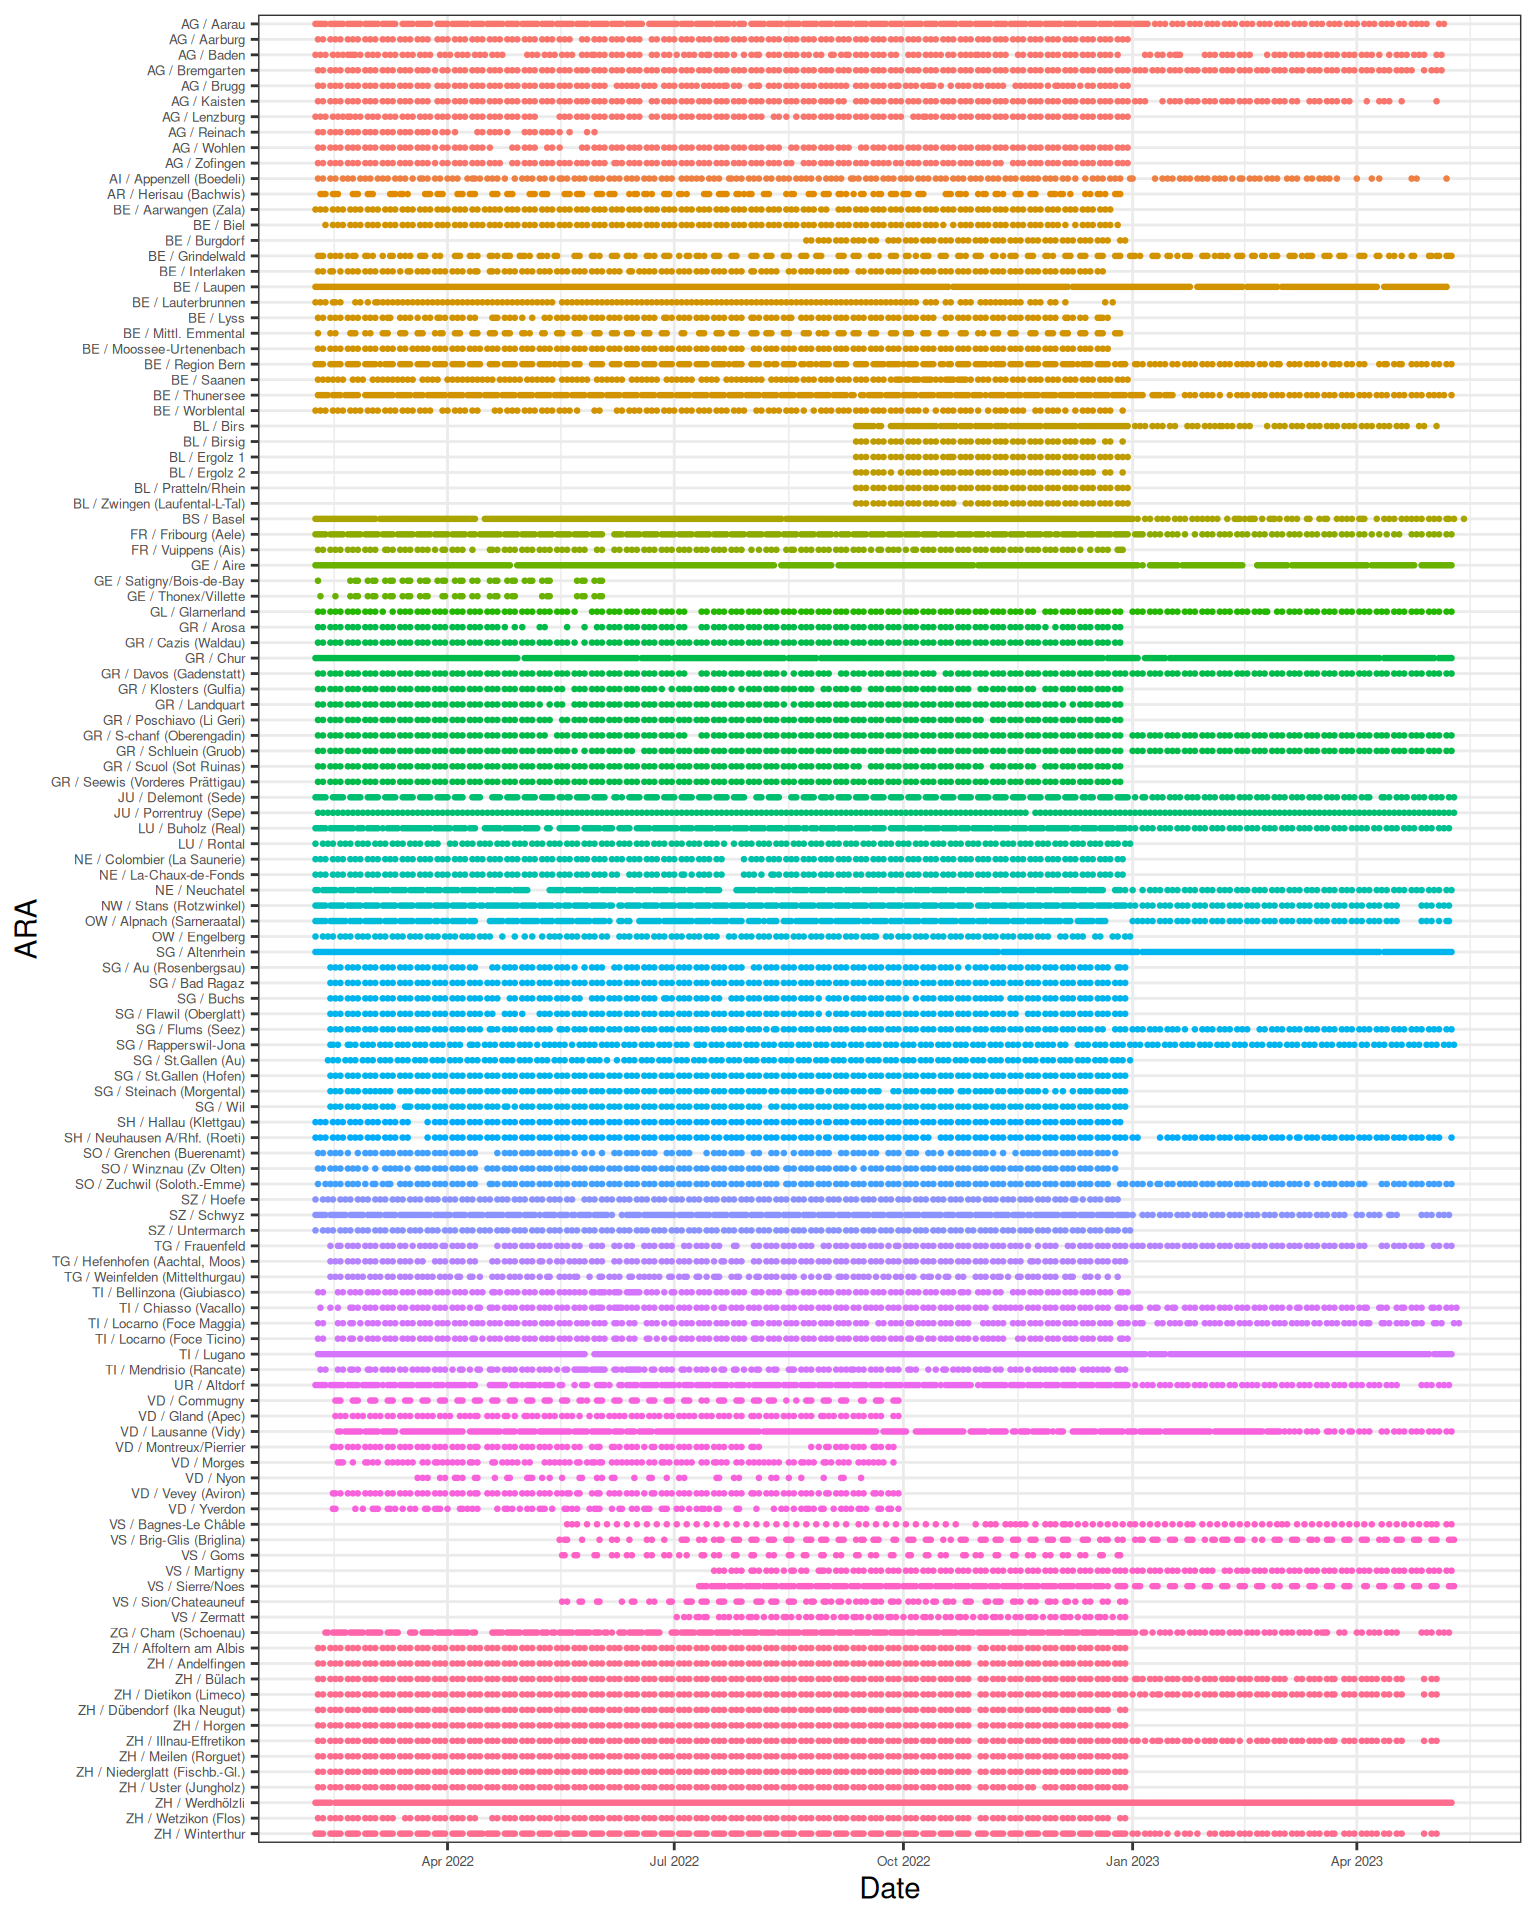
\includegraphics[width=.55\linewidth]{../reports/data_description_files/figure-html/fig1-1}
			\caption{Available measurements over time by ARA (coloured by canton).}
		\end{figure}
	\end{frame}
		
	\begin{frame}
		\frametitle{Data}
		\begin{figure}
			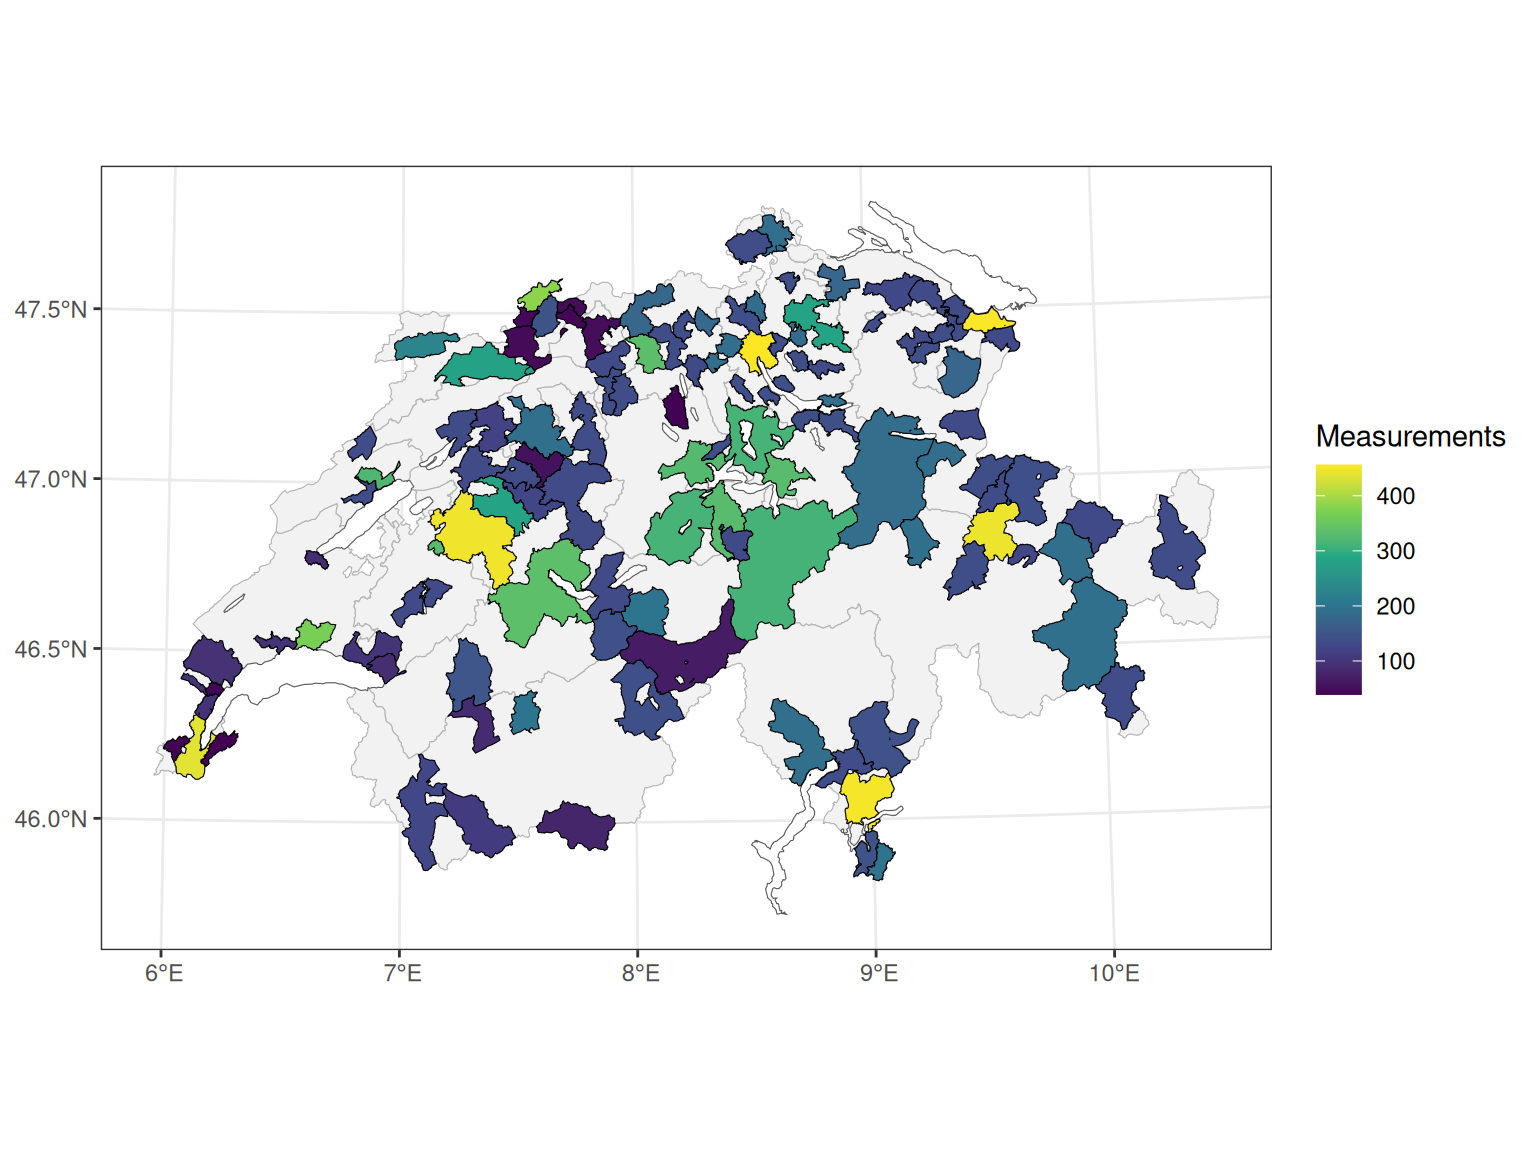
\includegraphics[width=.9\linewidth]{../reports/data_description_files/figure-html/map_missing-1}
			\vspace{-2em}
			\caption{Number of measurements by ARA.}
		\end{figure}
	\end{frame}
	
	\begin{frame}
		\frametitle{Data}
		
		Large \alert{heterogeneity} across time and space.
		\bigskip
		
		\begin{figure}
			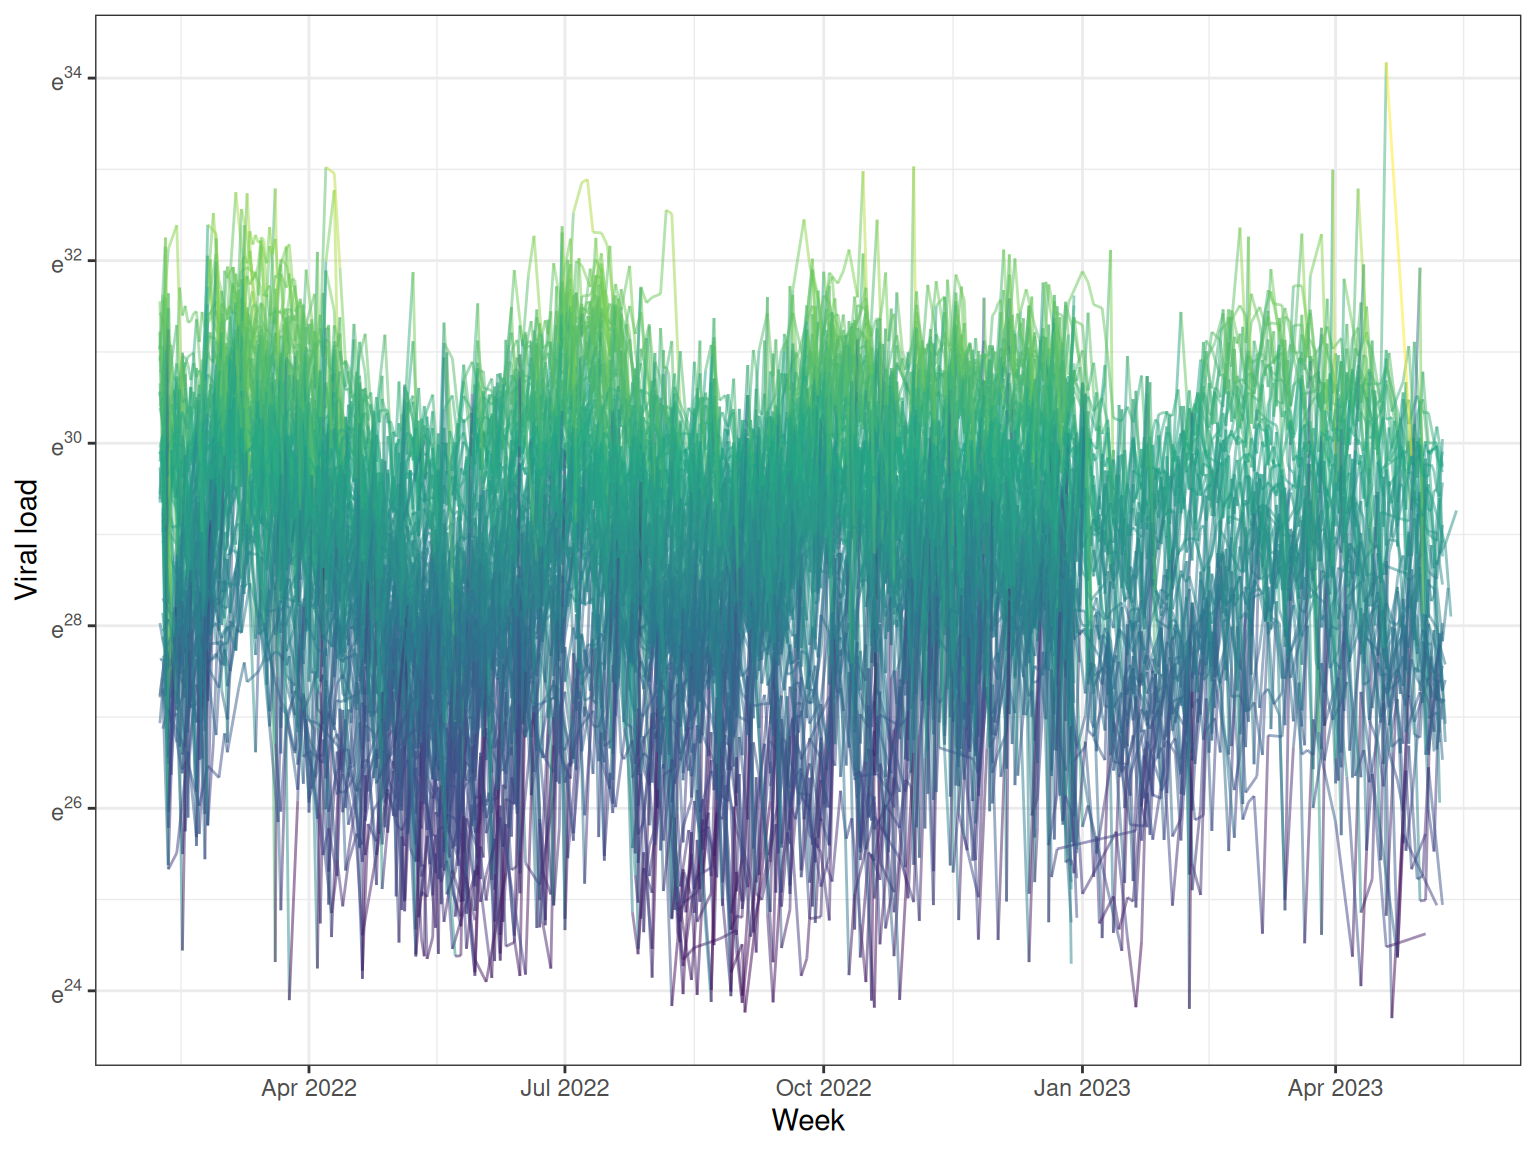
\includegraphics[width=.75\linewidth]{../reports/data_description_files/figure-html/fig_vl2-1}
			\caption{Daily SARS-CoV-2 viral load in wastewater by ARA (removing values below the LOD or LOQ).}
		\end{figure}
	\end{frame}
	
	\begin{frame}
		\frametitle{Objectives}
		1. Disentangle the \alert{various sources of heterogeneity}
		\begin{itemize}
			\item laboratory, quantification method, systematic temporal or spatial effects, remaining noise...
		\end{itemize}
		\pause\bigskip
		
		2. Extract a clean, ``noise-free'' \alert{temporal signal}
		\begin{itemize}
			\item at the national and/or regional level
		\end{itemize}
		\pause\bigskip
		
		3. Assess the \alert{agreement} with other types of surveillance 
		\begin{itemize}
			\item confirmed cases, hospitalisations...
		\end{itemize}
	\end{frame}
	
	\begin{frame}
		\frametitle{Method}
		\alert{Spatial regression} model using INLA accounting for:
		\begin{itemize}
			\item population covered \pause
			\item limits of detection (LOD) and of quantification (LOQ) \pause
			\item \alert{laboratory} and quantification method \pause
			\item systematic temporal effects (holidays, weekends) \pause
			\item \alert{systematic bias} by ARA 
			
		\end{itemize}
	\end{frame}
	
	
	\begin{frame}
		\frametitle{Method}
		Technical aspects:
		\begin{itemize}
			\item gamma likelihood (strictly positive)  \pause
			\item logarithmic link implying \alert{multiplicative effects} 
			$$ \log(V) = \alpha + X\beta \ \ \ \ \rightarrow \ \ \ \ V = \exp(\alpha) \times  \exp(X\beta)$$
			
			 \pause
			\item iterative model development (model selection tools) \pause
			\item \alert{random walks} for temporal trends \pause
			\item \alert{Besag-York-Mollié} for spatial correlation (neighbours)
			
		\end{itemize}
	\end{frame}
	
	\begin{frame}
		\frametitle{Results}
		\begin{figure}
			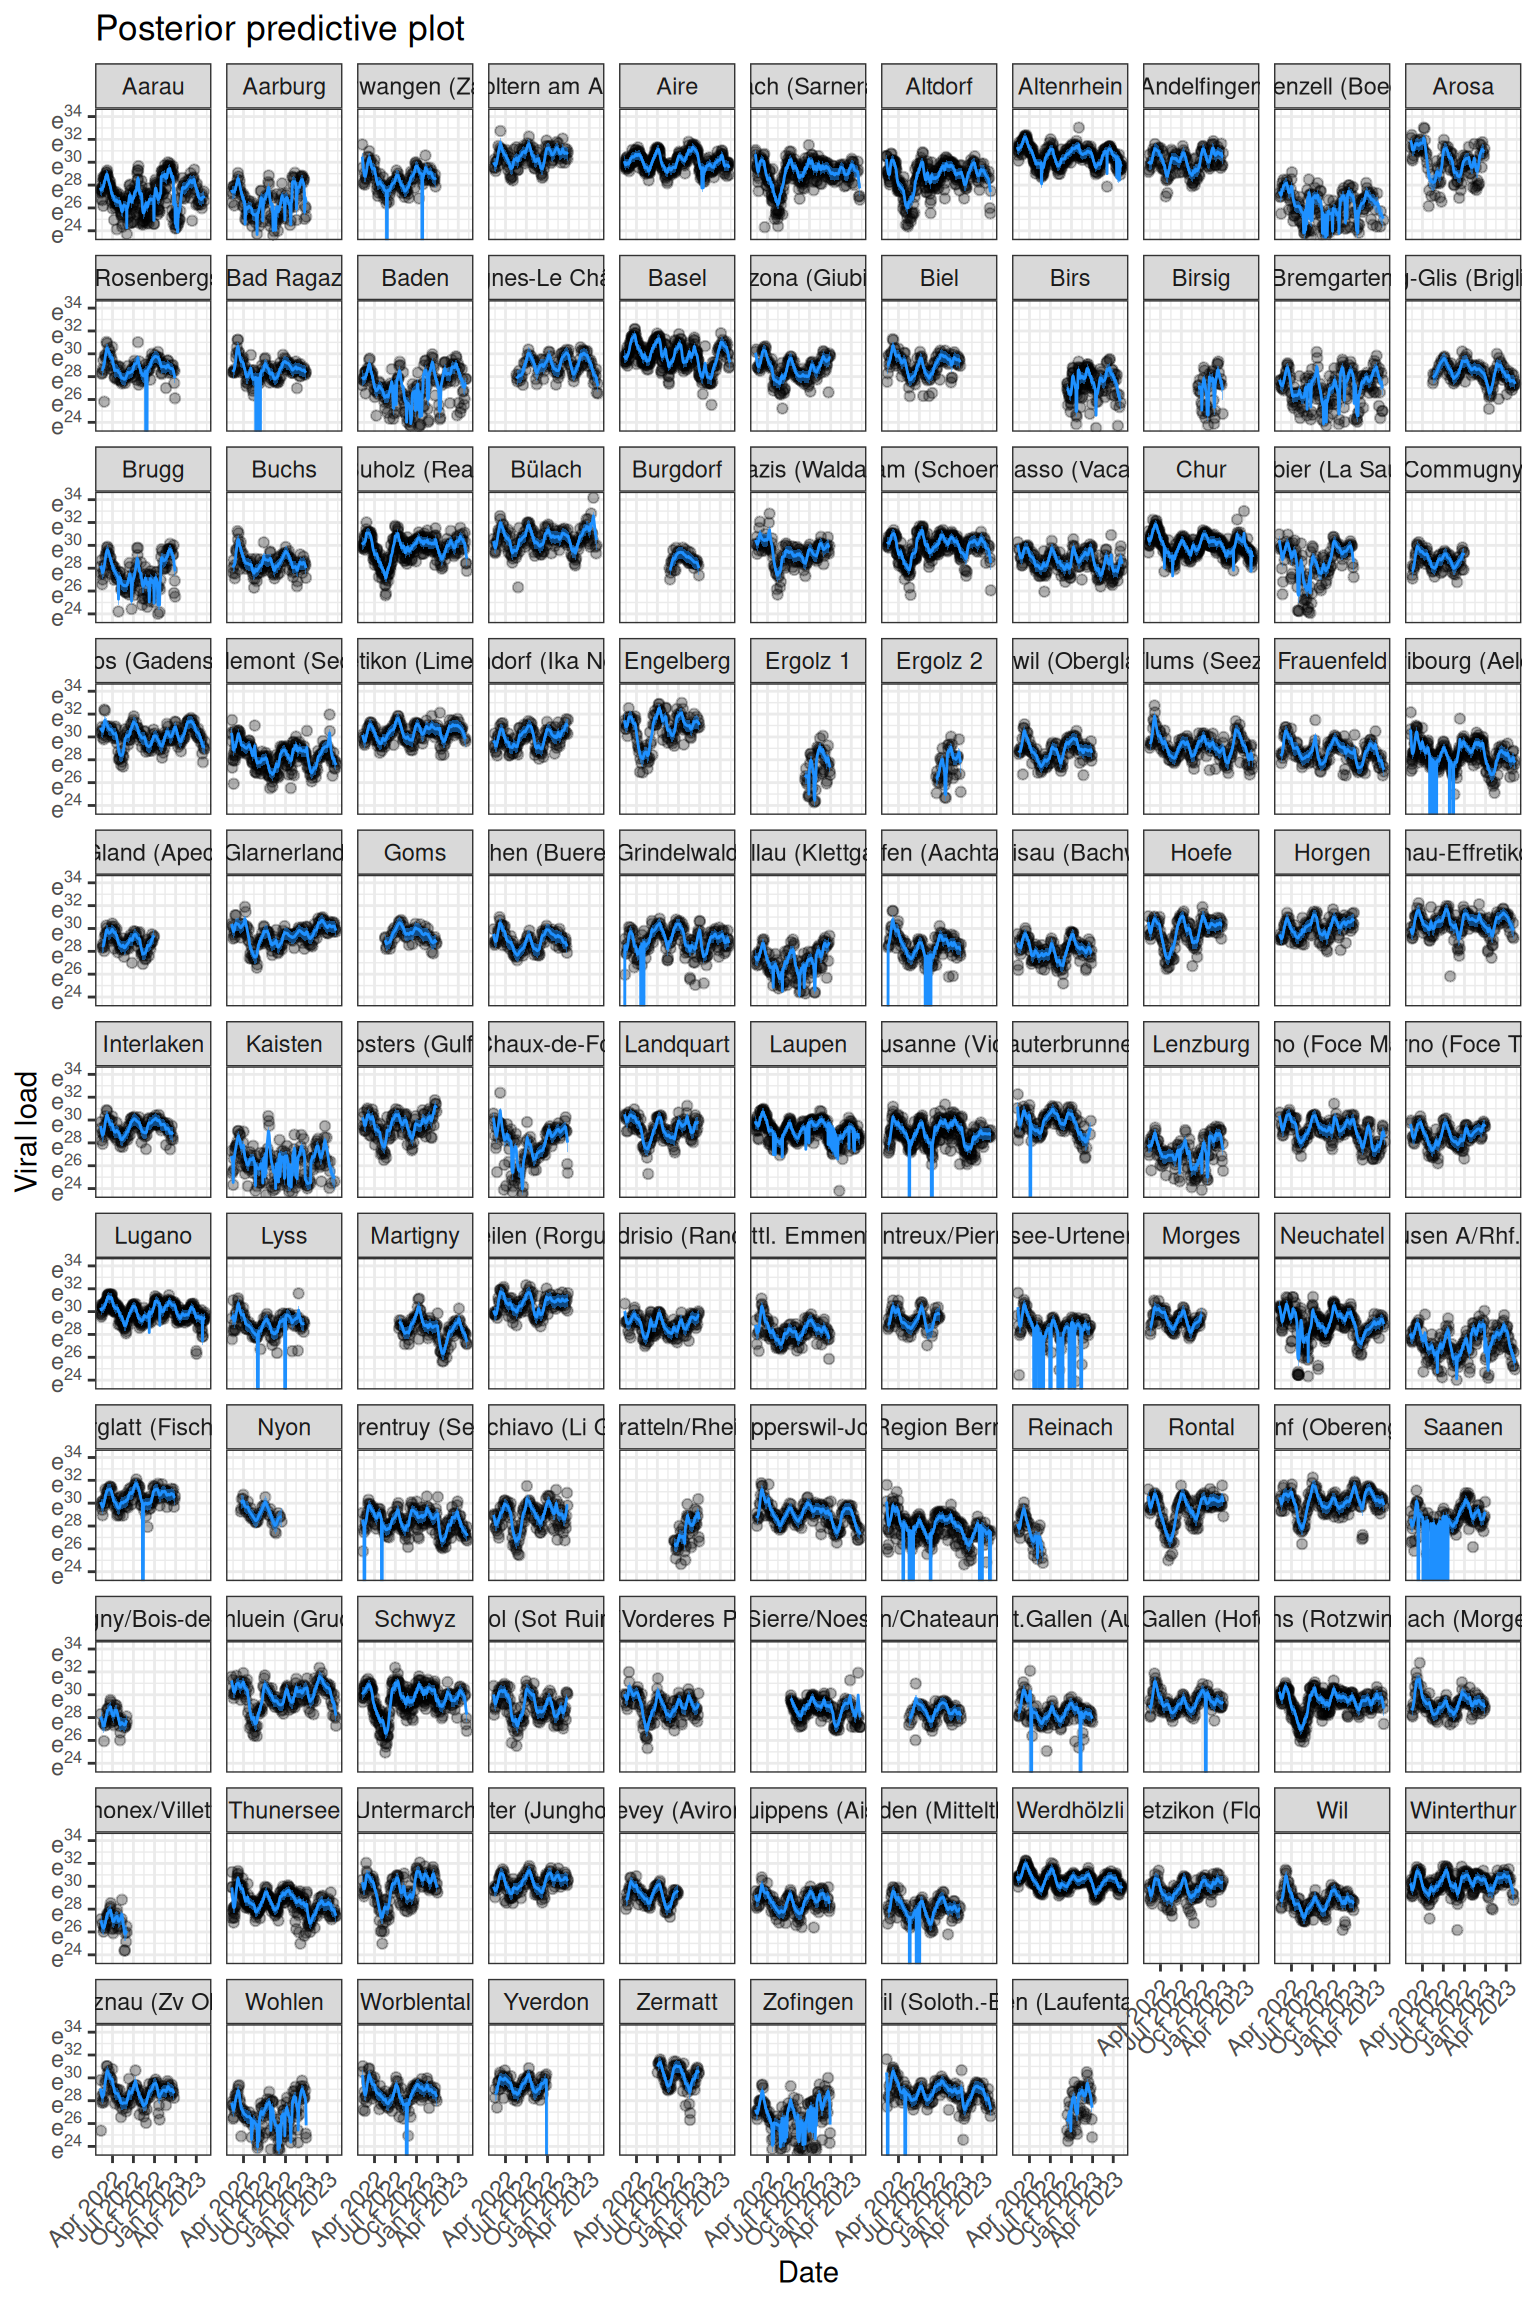
\includegraphics[width=0.5\linewidth]{../reports/model_dev_A3_files/figure-html/ma5.3.2a-1}
			\caption{Model fit}
		\end{figure}

%		
%		\begin{figure}
%			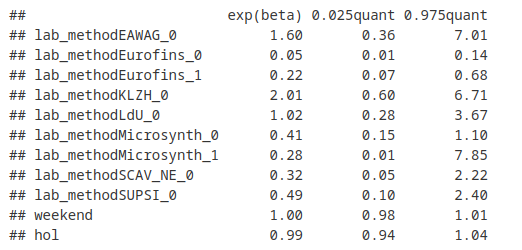
\includegraphics[width=0.7\linewidth]{figures/m5.3.2_res}
%			\caption{}
%			\label{fig:m5}
%		\end{figure}
		
	\end{frame}
	
\end{document}